\documentclass[12pt]{report}

\usepackage[a4paper,left=1.5in,right=1in,top=1in,bottom=1in,nohead]{geometry}
\usepackage{setspace}
\usepackage{mathptmx}
\usepackage{graphicx}
\usepackage{titlesec}
\usepackage{array}
\usepackage{booktabs}
\usepackage{longtable}
\usepackage{amsmath}
\usepackage{amssymb}
\usepackage{amsthm}
\usepackage{algorithm}
\usepackage{algpseudocode}
\usepackage{listings}
\usepackage{ragged2e}
\usepackage{rotating}
\usepackage{subcaption}
\usepackage{float}
\usepackage{hyperref}
\usepackage{xcolor}
\usepackage{multirow}
\usepackage{enumitem}

\setstretch{1.5}
\hypersetup{
    colorlinks=true,
    linkcolor=black,
    citecolor=black,
    urlcolor=blue
}

\renewcommand*\contentsname{\MakeUppercase{Table of Contents}}
\renewcommand{\listtablename}{List of Tables}
\renewcommand{\listfigurename}{List of Figures}

\titleformat{\chapter}[block]{\normalfont\Large\bfseries}{CHAPTER \thechapter}{0.3em}{\linebreak\centering\MakeUppercase}
\titlespacing*{\chapter}{0pt}{-1em}{0pt}
\titleformat{\section}[block]{\normalfont\bfseries}{\thesection}{0.3em}{\MakeUppercase}
\titleformat{\subsection}[block]{\normalfont\bfseries}{\thesubsection}{0.3em}{}

\lstset{
  basicstyle=\scriptsize\ttfamily,
  frame=tb,
  showstringspaces=false,
  keepspaces=true,
  breaklines=true,
  captionpos=b
}

\newcommand{\projecttitle}{QNA-Auth: Noise-Based Device Verification Using Multi-Source Sensor Fingerprints}
\newcommand{\studentname}{Your Name}
\newcommand{\regnumber}{Your Registration Number}
\newcommand{\guide}{Guide Name}
\newcommand{\department}{School of Computer Science and Engineering}
\newcommand{\institution}{Vellore Institute of Technology}
\newcommand{\submissionmonth}{April 2026}

\begin{document}
\pagestyle{plain}
\pagenumbering{roman}

\begin{titlepage}
    \centering
    \vspace*{1.2cm}
    {\Large\bfseries \projecttitle \par}
    \vspace{1.2cm}
    {\large A Project Report / Thesis Draft\par}
    \vspace{1.2cm}
    Submitted in partial fulfillment of the requirements for the award of the degree of\par
    \vspace{0.6cm}
    {\large\bfseries Bachelor of Technology\par}
    \vspace{0.6cm}
    in\par
    \vspace{0.4cm}
    {\large\bfseries Computer Science and Engineering\par}
    \vspace{1.4cm}
    Submitted by\par
    \vspace{0.4cm}
    {\large\bfseries \studentname\par}
    {\large \regnumber\par}
    \vspace{1.2cm}
    Under the guidance of\par
    \vspace{0.4cm}
    {\large\bfseries \guide\par}
    \vfill
    {\large \department\par}
    {\large \institution\par}
    \vspace{0.4cm}
    {\large \submissionmonth\par}
\end{titlepage}

\tableofcontents
\newpage

\chapter*{Executive Summary}
\addcontentsline{toc}{section}{Executive Summary}
\justifying
QNA-Auth is a capstone prototype for device verification based on the observation that camera and microphone pipelines expose measurable hardware- and environment-dependent noise characteristics. The project does not claim cryptographic identity or spoof-proof security. Instead, it treats learned embeddings as biometric-like feature templates that support repeated similarity matching under a bounded attacker model. This framing is important because raw embeddings are not used as credentials and the system is explicit about uncertainty, replay resistance, and drift.

The implemented system combines four major layers. First, the collection layer acquires camera and microphone noise samples either directly from runtime hardware or from client-provided arrays. Second, the preprocessing layer converts each sample into a fixed canonical feature vector using statistical, spectral, autocorrelation, entropy, and complexity descriptors. Third, a Siamese-style embedding network transforms the engineered feature vector into a normalized representation suitable for pairwise comparison. Fourth, the application layer performs enrollment, weighted multi-source fusion, confidence-band based authentication, margin checking against nearby impostors, and a nonce-bound challenge verification flow hardened with HKDF and a server secret.

The repository contains an end-to-end implementation with a FastAPI backend, SQLite-backed persistence for devices and challenges, evaluation scripts, a React frontend, and automated tests for threshold logic, multi-template handling, drift updates, and session split behavior. The latest review artifact in the repository, generated on April 22, 2026, uses a device-level split on microphone samples and reports a Siamese equal error rate of 0.10 under that constrained evaluation slice, with replay, impersonation, and synthetic-statistics attack success means reported as 0.0 in the same artifact. These numbers should be interpreted conservatively because the dataset scale is still limited. The main contribution of the project is therefore an end-to-end, security-aware verification pipeline that is technically coherent, review-ready, and extendable into stronger multi-session research.

\newpage
\listoftables
\addcontentsline{toc}{section}{List of Tables}
\newpage
\listoffigures
\addcontentsline{toc}{section}{List of Figures}
\newpage

\chapter*{List of Abbreviations}
\addcontentsline{toc}{section}{List of Abbreviations}
\begin{longtable}{p{0.18\textwidth}p{0.72\textwidth}}
\textbf{AI} & Artificial Intelligence \\
\textbf{API} & Application Programming Interface \\
\textbf{ASR} & Attack Success Rate \\
\textbf{AUC} & Area Under Curve \\
\textbf{CNN} & Convolutional Neural Network \\
\textbf{DB} & Database \\
\textbf{EER} & Equal Error Rate \\
\textbf{EMA} & Exponential Moving Average \\
\textbf{FAR} & False Acceptance Rate \\
\textbf{FRR} & False Rejection Rate \\
\textbf{FFT} & Fast Fourier Transform \\
\textbf{HKDF} & HMAC-based Key Derivation Function \\
\textbf{HMAC} & Hash-based Message Authentication Code \\
\textbf{JSON} & JavaScript Object Notation \\
\textbf{ML} & Machine Learning \\
\textbf{PR} & Precision-Recall \\
\textbf{PUF} & Physical Unclonable Function \\
\textbf{ROC} & Receiver Operating Characteristic \\
\textbf{RMS} & Root Mean Square \\
\textbf{SNR} & Signal-to-Noise Ratio \\
\textbf{SQL} & Structured Query Language \\
\textbf{UI} & User Interface \\
\end{longtable}

\newpage
\chapter*{List of Symbols}
\addcontentsline{toc}{section}{List of Symbols}
\begin{longtable}{p{0.18\textwidth}p{0.72\textwidth}}
$x$ & Input feature vector extracted from one sensor-noise sample \\
$f_{\theta}(x)$ & Learned embedding function parameterized by network weights $\theta$ \\
$e_i$ & Embedding corresponding to the $i^{th}$ sample \\
$s(e_a, e_b)$ & Similarity score between embeddings $e_a$ and $e_b$ \\
$w_c, w_m$ & Source fusion weights for camera and microphone respectively \\
$\tau_s$ & Strong accept threshold \\
$\tau_u$ & Uncertain threshold \\
$m$ & Required identification margin against the closest impostor \\
$\alpha$ & EMA drift update coefficient \\
$\mathcal{L}_{triplet}$ & Triplet loss used for metric learning \\
$\mu$ & Mean of a feature distribution \\
$\sigma$ & Standard deviation of a feature distribution \\
\end{longtable}

\newpage
\pagenumbering{arabic}
\setcounter{page}{1}

\chapter{Introduction}
\justifying
\section{Background}
Digital authentication systems traditionally rely on something the user knows, such as a password, or something the user possesses, such as a token or mobile device. Both categories are practical, but both expose familiar failure modes: passwords are phishable and reusable, tokens can be stolen or replayed, and static device identifiers are often easy to clone. This project explores a third signal family: whether stochastic noise characteristics produced by sensors can serve as a repeatable verification cue for the same physical device.

QNA-Auth approaches this problem through camera and microphone noise. Camera capture introduces sensor artifacts and acquisition pipeline characteristics. Microphone recordings carry analog front-end noise, quantization artifacts, gain behavior, and environmental signatures. Neither source alone is assumed to be perfectly stable or unique, but both may contain enough structure to support high-confidence matching when processed carefully. The project therefore treats device verification as a probabilistic similarity task rather than an identity claim.

The theoretical basis combines engineered feature extraction with metric learning. Each raw sample is reduced to a canonical feature vector containing time-domain statistics, spectral measures, entropy, autocorrelation descriptors, and complexity metrics. A Siamese-style embedding model then learns a representation in which samples from the same device are expected to be closer than samples from different devices. Similarity is measured by cosine similarity on normalized embeddings, which yields an operational decision score.

\subsection{Need for a Structured Security Framing}
Sensor-based verification is easy to overstate. A strong thesis must explicitly separate what the prototype does from what it does not do. This repository already reflects that discipline. The README and runtime metadata consistently frame embeddings as feature templates used only for similarity. They are not stored or used as standalone credentials. The project also recognizes that environmental shifts can move genuine samples into an uncertain band, and that adaptive attackers remain a residual risk. This thesis adopts the same language because a rigorous report must align with the system's true guarantees.

\subsection{Why Multi-Source Verification}
Single-source biometric or device signals often fail because they overfit one fragile measurement path. QNA-Auth reduces that fragility by combining camera and microphone embeddings at decision time using weighted fusion. The current configuration gives camera a weight of 0.7 and microphone a weight of 0.3. That choice reflects an engineering assumption embodied in the code rather than a universal truth: the stronger source receives higher influence, while the secondary source contributes robustness when its measurements are consistent.

\section{Motivation}
The primary motivation is practical. A capstone project should demonstrate a complete technical system, not just isolated scripts. QNA-Auth satisfies that requirement by joining data collection, preprocessing, learned embeddings, verification logic, secure challenge handling, persistence, evaluation, and user interface layers into one deployable prototype.

There is also an academic motivation. Device verification through sensor noise sits at the intersection of signal processing, machine learning, and applied security. It allows the project to discuss feature engineering, metric learning, score calibration, attack models, confidence bands, and system-level limitations in a unified setting. This makes the work suitable for a thesis because it is both implementation-heavy and analytically rich.

Finally, there is a review-day motivation. The repository includes a clear live-demo workflow, preflight diagnostics, and reviewer-safe language. That is not incidental. A technically sound thesis must also support reproducibility, explanation, and controlled demonstration. The project was shaped with that constraint in mind.

\section{Scope of the Project}
The functional scope of QNA-Auth includes device enrollment, authentication against an enrolled template, challenge creation, challenge verification, device listing, device metadata inspection, and device deletion. The system supports two active runtime sources: camera and microphone. Older references to QRNG remain in some historical documentation, but the active verification pipeline uses only camera and microphone signals.

The technical scope includes a FastAPI backend, a PyTorch embedding model, shared preprocessing code for training and runtime, SQLite-backed persistence, React-based frontend pages for home, enrollment, authentication, and device management, plus reporting and diagnostic scripts. The report also covers evaluation tooling, split policies, and attack-surface documentation.

The boundaries of the project are equally important:
\begin{itemize}[leftmargin=1.2cm]
\item The system is a prototype for high-confidence device matching, not a replacement for cryptographic identity.
\item Performance is dependent on dataset quality, number of devices, and environmental conditions.
\item The challenge-response flow hardens verification against replay but does not establish a full client-side secret possession model.
\item Real-world deployment concerns such as hardware diversity, liveness, secure enclaves, and large-scale threshold calibration are outside the implemented scope.
\end{itemize}

\section{Problem Statement}
The core problem addressed by this thesis is: \emph{Can a software system use camera and microphone sensor noise to produce repeatable, security-aware device verification decisions, while remaining honest about uncertainty and implementation limits?}

This problem has three sub-parts. First, the system must convert noisy, variable-length sensor captures into stable fixed-size numerical representations. Second, it must learn a similarity space in which genuine device samples are closer than impostor samples. Third, it must expose those decisions through a controlled application workflow that resists simple replay, explains uncertainty, and stores reproducible metadata.

\section{Contributions}
The main contributions of this project are as follows:
\begin{itemize}[leftmargin=1.2cm]
\item A complete end-to-end implementation for noise-based device verification using camera and microphone inputs.
\item A shared feature extraction pipeline used consistently across training, evaluation, enrollment, and runtime authentication.
\item Weighted multi-source template fusion, confidence bands, source-profile guards, template-bank scoring, and nearest-impostor margin checks.
\item A nonce-bound challenge verification flow hardened with HKDF and a server secret.
\item A review-ready software package with API endpoints, database persistence, frontend, diagnostics, evaluation scripts, and reporting helpers.
\end{itemize}

\chapter{Project Description and Goals}
\section{Literature Review}
Similarity learning with twin or shared-weight networks has been an established direction since early work on Siamese neural networks for signature verification \cite{bromley1993signature}. Later work on contrastive and triplet-based objectives further strengthened the view that representation learning can be optimized directly for closeness of same-class samples and separation of different-class samples \cite{hadsell2006dimensionality, schroff2015facenet}. QNA-Auth follows this family of ideas, but applies them to fixed engineered features instead of raw images or waveform segments.

Feature extraction from noisy measurements remains relevant even in deep learning pipelines. Signal-processing descriptors such as mean, variance, entropy, power distribution, and frequency-domain statistics compress raw measurements while preserving useful discriminatory information. Shannon's information framework motivates entropy-based measures \cite{shannon1948mathematical}, while classical spectral estimation methods motivate frequency-domain analysis \cite{welch1967use}. In this repository, feature engineering serves two purposes: it makes the runtime pipeline lightweight, and it provides interpretable intermediate quantities that are easier to debug than opaque raw-input models.

The project also draws from authentication-system design rather than only pattern recognition. Modern security practice emphasizes threat models, replay protection, bounded claims, and failure handling. QNA-Auth reflects this through challenge expiry, nonce binding, optional API keys, rate limiting, and audit logging. This is a meaningful distinction from a pure classification exercise: the system is not evaluated only by its embedding quality, but also by how safely it exposes that embedding logic through an API.

\section{Research Gap}
The gap addressed by QNA-Auth is not that sensor fingerprints are an entirely new idea, but that many student-level implementations stop at one of two extremes. Some remain at the proof-of-concept stage, producing one-off similarity scores without a deployable service layer. Others build application interfaces without a defensible signal-processing or security story.

This project attempts to close that gap in five specific ways:
\begin{itemize}[leftmargin=1.2cm]
\item It unifies collection, feature extraction, learned embeddings, persistence, API exposure, and UI into one coherent repository.
\item It frames uncertainty explicitly through strong, uncertain, and reject bands instead of a single unqualified binary threshold.
\item It adds a nearest-impostor margin guard so that a claimed-device score is not accepted purely because it exceeds a threshold.
\item It stores metadata about source profiles, template banks, and drift updates to support explanation and later analysis.
\item It hardens the two-step challenge flow so that a captured response cannot be replayed across requests without also reproducing the stable feature template under a fresh nonce.
\end{itemize}

\section{Objectives}
The project objectives can be stated precisely:
\begin{enumerate}[leftmargin=1.2cm]
\item Build a reusable pipeline that captures camera and microphone noise and converts it into a fixed canonical feature vector.
\item Train or load a Siamese-style embedding model that maps feature vectors into a normalized similarity space.
\item Support multi-source device enrollment and weighted source fusion at authentication time.
\item Expose the system through a FastAPI backend and React frontend suitable for demonstration and inspection.
\item Add security-aware controls such as nonce-bound verification, rate limiting, confidence bands, and audit logging.
\item Evaluate the approach using device-level splits, threshold sweeps, ROC/PR analysis, and attacker-oriented metrics from repository artifacts.
\end{enumerate}

\section{Project Plan}
The software repository suggests a staged plan that is appropriate for a thesis narrative:
\begin{itemize}[leftmargin=1.2cm]
\item Phase 1: establish data collection and preprocessing consistency.
\item Phase 2: implement embedding generation and training/evaluation scripts.
\item Phase 3: create enrollment and authentication workflows with persistence.
\item Phase 4: introduce security hardening, review-time safeguards, and frontend usability.
\item Phase 5: perform evaluation, document limitations, and prepare demo/review material.
\end{itemize}

The presence of dedicated folders such as \texttt{scripts/training}, \texttt{scripts/diagnostics}, and \texttt{scripts/reporting}, along with review-specific documentation in \texttt{docs/}, confirms that the project evolved as a structured software system rather than as a monolithic experimental notebook.

\section{Expected Outcomes}
The expected outcome is not perfect device identity but an operational prototype that can:
\begin{itemize}[leftmargin=1.2cm]
\item enroll a device from multiple sensor-noise samples,
\item verify subsequent samples against stored templates,
\item separate strong matches from ambiguous cases,
\item reject simple replay through challenge hardening,
\item expose interpretable metrics and logs for analysis.
\end{itemize}

\chapter{Technical Specification}
\section{System Requirements}
\subsection{Functional Requirements}
The repository and backend implementation imply the following functional requirements:
\begin{itemize}[leftmargin=1.2cm]
\item The system shall enroll a device and create a persistent template bundle.
\item The system shall authenticate a claimed device using fresh camera and/or microphone samples.
\item The system shall create a short-lived challenge and verify a response bound to a nonce.
\item The system shall store device metadata, active challenges, and audit log events in a database.
\item The system shall allow inspection, listing, and deletion of enrolled devices.
\item The frontend shall provide enrollment, authentication, and device-management pages.
\end{itemize}

\subsection{Non-Functional Requirements}
Important non-functional requirements are performance consistency, reproducibility, explainability, and review safety. The code shows deliberate engineering in these areas: configuration is centralized in \texttt{config.py}, the feature pipeline is versioned, thresholds are explicit, and runtime counters are exposed through a \texttt{/stats} endpoint. Reproducibility is strengthened by artifact generation under \texttt{artifacts/capstone\_eval/} and by metadata stored alongside each embedding.

\subsection{Hardware and Software Stack}
Table \ref{tab:stack} summarizes the implemented stack.

\begin{table}[H]
\centering
\caption{Technology stack used in QNA-Auth}
\label{tab:stack}
\renewcommand{\arraystretch}{1.3}
\begin{tabular}{p{0.24\textwidth}p{0.26\textwidth}p{0.36\textwidth}}
\toprule
\textbf{Layer} & \textbf{Technology} & \textbf{Purpose} \\
\midrule
Backend API & FastAPI, Pydantic & REST endpoints, request validation, runtime orchestration \\
Modeling & PyTorch & Embedding network and similarity computation \\
Preprocessing & NumPy, SciPy & Feature extraction from raw noise arrays \\
Persistence & SQLite, SQLAlchemy & Devices, challenges, and audit logs \\
Frontend & React, TypeScript, Vite & Enrollment/authentication UI \\
Diagnostics & Python scripts & Preflight checks, reporting, evaluation helpers \\
\bottomrule
\end{tabular}
\end{table}

\section{Feasibility Study}
\subsection{Technical Feasibility}
The project is technically feasible because all major operations can run on commodity hardware. The feature extraction pipeline works on one-dimensional arrays and avoids requiring large end-to-end raw-input neural architectures. The backend can run with CPU inference if GPU acceleration is unavailable. The database layer uses SQLite by default, which is sufficient for a capstone prototype.

\subsection{Operational Feasibility}
Operationally, the project is feasible for demo and academic evaluation because it includes a preflight script, fallback demo workflow, and a review brief generator. This reduces the risk that hardware instability during live presentation will invalidate the system narrative.

\subsection{Research Feasibility}
Research feasibility is moderate but bounded. The repository already contains evaluation scripts, attack summaries, and split artifacts. However, the current dataset remains relatively small, so the thesis must avoid overclaiming generalization. The project is therefore feasible as a prototype-and-evaluation thesis, not yet as a final claim of broad deployment performance.

\section{Feature and Embedding Specification}
The canonical feature extractor in \texttt{preprocessing/features.py} produces a versioned feature set composed of raw-domain and normalized-domain attributes. These include:
\begin{itemize}[leftmargin=1.2cm]
\item raw statistics: mean, standard deviation, variance, range, quartiles, RMS, peak factor;
\item information content: Shannon entropy;
\item spectral descriptors: dominant frequency, dominant magnitude, spectral centroid, spread, entropy, flatness, and band powers;
\item autocorrelation descriptors: first zero crossing, mean autocorrelation windows, decay trend;
\item complexity descriptors: zero-crossing rate, approximate entropy, and Hurst exponent.
\end{itemize}

If $x \in \mathbb{R}^{d}$ is a feature vector and $f_{\theta}$ is the learned embedding function, the normalized embedding is:
\begin{equation}
e = \frac{f_{\theta}(x)}{\left\lVert f_{\theta}(x) \right\rVert_2}
\end{equation}

Similarity between two embeddings is computed using cosine similarity:
\begin{equation}
s(e_a, e_b) = \frac{e_a \cdot e_b}{\left\lVert e_a \right\rVert_2 \left\lVert e_b \right\rVert_2}
\end{equation}

For multi-source fusion, the repository combines source embeddings using normalized weights:
\begin{equation}
e_{combined} = \frac{w_c e_{camera} + w_m e_{microphone}}{\left\lVert w_c e_{camera} + w_m e_{microphone} \right\rVert_2}
\end{equation}
where currently $w_c = 0.7$ and $w_m = 0.3$.

\section{Decision Policy}
The runtime decision policy is intentionally richer than a single threshold. Let $\tau_s$ denote the strong accept threshold and $\tau_u$ the uncertain threshold, with $\tau_s > \tau_u$. The current configuration sets:
\begin{equation}
\tau_s = 0.97,\hspace{1cm}\tau_u = 0.92
\end{equation}

Decision logic is:
\begin{itemize}[leftmargin=1.2cm]
\item if $s \geq \tau_s$, the sample enters the strong-accept band;
\item if $\tau_u \leq s < \tau_s$, the sample is marked uncertain and may require more samples or fallback authentication;
\item if $s < \tau_u$, the sample is rejected.
\end{itemize}

Acceptance also depends on an identification margin:
\begin{equation}
s_{claimed} - s_{best\_other} \geq m
\end{equation}
where the configured margin is $m = 0.02$. This prevents acceptance when a claimed-device score is only marginally better than the nearest impostor.

\section{Dataset and Split Specification}
The repository documentation recommends research-level evaluation with versioned datasets, session metadata, and split tracking. The latest artifact included in the repository uses a device-level split for microphone records with counts shown in Table \ref{tab:splitcounts}.

\begin{table}[H]
\centering
\caption{Counts from the device split artifact dated April 22, 2026}
\label{tab:splitcounts}
\renewcommand{\arraystretch}{1.3}
\begin{tabular}{lcc}
\toprule
\textbf{Split} & \textbf{Records} & \textbf{Purpose} \\
\midrule
Train & 22 & Model fitting and threshold search support \\
Validation & 10 & Tuning and intermediate inspection \\
Test & 8 & Final reported slice in the artifact \\
\bottomrule
\end{tabular}
\end{table}

These numbers are sufficient for a prototype demonstration but not for broad claims. The thesis should therefore use the results as evidence of pipeline behavior under a documented setup, not as evidence of production readiness.

\chapter{System Design}
\section{System Architecture}
QNA-Auth follows a layered architecture. Figure \ref{fig:architecture} summarizes the conceptual flow.

\begin{figure}[H]
\centering
\fbox{
\begin{minipage}{0.9\textwidth}
\centering
\vspace{0.4cm}
\textbf{Client / Frontend} \\
React pages for Home, Enroll, Authenticate, Devices \\
\vspace{0.2cm}
$\downarrow$ \\
\vspace{0.2cm}
\textbf{API Layer} \\
FastAPI endpoints: \texttt{/enroll}, \texttt{/authenticate}, \texttt{/challenge}, \texttt{/verify}, \texttt{/devices} \\
\vspace{0.2cm}
$\downarrow$ \\
\vspace{0.2cm}
\textbf{Application Logic} \\
Enrollment, authentication, challenge hardening, thresholding, drift updates \\
\vspace{0.2cm}
$\downarrow$ \\
\vspace{0.2cm}
\textbf{Signal and Model Layer} \\
Noise collection, feature extraction, feature vector conversion, embedding model \\
\vspace{0.2cm}
$\downarrow$ \\
\vspace{0.2cm}
\textbf{Persistence and Artifacts} \\
SQLite DB, device template files, audit logs, evaluation results \\
\vspace{0.4cm}
\end{minipage}
}
\caption{Conceptual architecture of QNA-Auth}
\label{fig:architecture}
\end{figure}

The design is intentionally modular. The \texttt{server/} package owns HTTP concerns, the \texttt{auth/} package owns enrollment and authentication logic, \texttt{preprocessing/} owns feature extraction, \texttt{model/} owns embeddings and evaluation, and \texttt{db/} owns persistence. This separation matters because it allows the same preprocessing and embedding code to be reused consistently across training and runtime.

\section{Detailed Design}
\subsection{Backend API Design}
The backend is instantiated in \texttt{server/app.py}. During startup, it loads source-specific models if configured, otherwise it falls back to a shared model path. It initializes the feature converter, database, device enroller, authenticator, challenge protocol, and secure authentication flow. This startup sequence ensures that request handlers do not need to rebuild heavy state for each request.

The principal endpoints are listed in Table \ref{tab:endpoints}.

\begin{table}[H]
\centering
\caption{Core API endpoints}
\label{tab:endpoints}
\renewcommand{\arraystretch}{1.3}
\begin{tabular}{p{0.22\textwidth}p{0.18\textwidth}p{0.46\textwidth}}
\toprule
\textbf{Endpoint} & \textbf{Method} & \textbf{Purpose} \\
\midrule
\texttt{/health} & GET & Health and initialization status \\
\texttt{/stats} & GET & Runtime counters and confidence-band totals \\
\texttt{/enroll} & POST & Enroll a new device and persist template bundle \\
\texttt{/authenticate} & POST & Perform direct similarity-based authentication \\
\texttt{/challenge} & POST & Create a short-lived nonce-bound challenge \\
\texttt{/verify} & POST & Verify challenge response and similarity band \\
\texttt{/devices} & GET & List enrolled devices \\
\texttt{/devices/\{device\_id\}} & GET/DELETE & Inspect or remove a device \\
\bottomrule
\end{tabular}
\end{table}

\subsection{Enrollment Design}
Enrollment starts with a set of raw samples grouped by source. For each source, the system extracts a feature vector for each sample, generates source embeddings, and aggregates them through a mean strategy. It also builds a template bank by chunking samples into smaller groups and averaging each chunk. This makes later scoring more robust than comparing against a single enrollment vector.

Metadata is stored alongside the template bundle. This includes sample counts, active sources, feature dimension, source RMS profiles, source weights, template strategy, drift-model configuration, and attacker-model notes. Such metadata is essential in a thesis because it makes the runtime behavior inspectable and reproducible.

\subsection{Authentication Design}
Authentication first checks whether the requested sources match those used during enrollment. It then validates basic source-profile consistency using RMS statistics. If the runtime samples differ too sharply from the enrolled RMS profile, authentication is rejected before similarity comparison. Otherwise, the system generates an authentication profile and scores it against the stored template bank.

Per-source scores are combined using configured weights. The system records per-source similarity, per-source band, strong and uncertain thresholds, template count, and template max similarity. After weighted fusion, the system computes the nearest-impostor margin across all enrolled devices. Only when the score falls in the strong-accept band, the margin is adequate, and no source check fails does the request authenticate successfully.

\subsection{Challenge-Response Design}
The challenge module adds a nonce-bound verification step. A challenge contains a device identifier, nonce, creation time, and expiry time. The MAC key is derived using HKDF over three inputs: a coarse quantized stable feature template, the nonce, and a server secret. This is a stronger design than directly using an embedding as a credential because the embedding never becomes a reusable secret. The flow also uses single-use challenges, so replaying an old response is not sufficient.

\subsection{Persistence Design}
The SQLAlchemy schema defines three entities: \texttt{Device}, \texttt{Challenge}, and \texttt{AuditLog}. The \texttt{Device} table stores device identifier, optional display name, path to embedding files, serialized metadata, and creation timestamp. The \texttt{Challenge} table persists active challenges so that the protocol is not limited to in-memory state. The \texttt{AuditLog} table records enrollment, authentication, challenge creation, verification, and deletion actions for later inspection.

\subsection{Frontend Design}
The React frontend is intentionally small and task-focused. The navigation exposes Home, Enroll, Authenticate, and Devices pages. The API client centralizes requests to the backend and defines TypeScript request and response interfaces. This improves demo usability and shows that the project is more than a command-line experiment.

\chapter{Methodology and Testing}
\section{Methodology}
\subsection{Noise Acquisition}
The enrollment and authentication flows support two acquisition modes. In the first mode, the backend directly samples hardware using the camera and microphone collectors. In the second mode, the client provides captured arrays through the API. The second mode is valuable for fallback demonstrations, regression testing, and review reproducibility.

Camera samples are obtained by capturing frames and extracting noise-oriented features from the image data. Microphone samples are captured as short-duration ambient recordings. Unsupported sources are explicitly ignored in the runtime enrollment path, which matches the current project scope.

\subsection{Preprocessing and Feature Extraction}
The preprocessing pipeline begins by reshaping raw arrays into one-dimensional floating-point signals and replacing invalid values. It then centers the sample, optionally normalizes it, and computes both raw-domain and normalized-domain features. This dual representation is important: raw features preserve amplitude-dependent information, while normalized features emphasize shape and spectral structure.

The feature extractor can also operate in a fast mode that reduces the analysis burden for expensive transforms. This is useful during live demos when stable latency matters more than maximal feature richness.

\subsection{Embedding Learning}
The embedding model is implemented as a multilayer perceptron inside a Siamese wrapper. Hidden layers use \texttt{Tanh} activations and produce a normalized embedding of dimension 128 by default. The repository contains both triplet-loss and contrastive-loss implementations, supporting metric-learning style training and experimentation \cite{hadsell2006dimensionality, schroff2015facenet}.

The triplet loss can be written as:
\begin{equation}
\mathcal{L}_{triplet} = \max \left(0, \lVert e_a - e_p \rVert_2 - \lVert e_a - e_n \rVert_2 + \gamma \right)
\end{equation}
where $e_a$, $e_p$, and $e_n$ denote anchor, positive, and negative embeddings, and $\gamma$ is the margin hyperparameter.

\subsection{Template Construction}
Enrollment does not rely on a single sample. Instead, multiple feature vectors are embedded and aggregated into:
\begin{itemize}[leftmargin=1.2cm]
\item a source embedding per modality,
\item a source template bank built from chunked sample groups,
\item a combined embedding,
\item a combined template bank obtained from source-template fusion.
\end{itemize}

This design supports more stable scoring because runtime authentication can compare against several enrollment templates rather than against one brittle vector.

\subsection{Confidence Bands and Drift Handling}
Confidence bands split decisions into strong accept, uncertain, and reject. This is preferable to a single hard threshold because real sensor noise can vary across sessions and environments. An uncertain result gives the system a safe middle state rather than forcing a false accept or false reject.

The system also supports rolling re-enrollment. If a request lands in the strong-accept band and drift updates are enabled, the template can be updated using an EMA rule:
\begin{equation}
e_{new} = \frac{(1-\alpha)e_{old} + \alpha e_{auth}}{\left\lVert (1-\alpha)e_{old} + \alpha e_{auth} \right\rVert_2}
\end{equation}
The code additionally requires a minimum number of strong accepts before applying the update, reducing the risk of gradual poisoning.

\section{Algorithms}
Algorithm \ref{alg:enroll} summarizes the enrollment flow implemented in the repository.

\begin{algorithm}[H]
\caption{Multi-source device enrollment}
\label{alg:enroll}
\begin{algorithmic}[1]
\Require Requested sources $S$, number of samples $N$
\Ensure Persisted template bundle and metadata
\State Collect or receive raw samples grouped by source
\ForAll{$s \in S$}
    \State Extract canonical feature vectors for source $s$
    \State Generate source embeddings from the feature vectors
    \State Build chunk-based template bank for source $s$
\EndFor
\State Fuse source embeddings using configured source weights
\State Fuse template banks into combined templates
\State Compute source RMS profiles and metadata
\State Persist embedding payload and metadata bundle
\end{algorithmic}
\end{algorithm}

Algorithm \ref{alg:auth} summarizes runtime authentication.

\begin{algorithm}[H]
\caption{Authentication with confidence bands and margin guard}
\label{alg:auth}
\begin{algorithmic}[1]
\Require Claimed device $d$, runtime samples, thresholds $\tau_s$, $\tau_u$, margin $m$
\Ensure Authentication decision and diagnostics
\State Load stored template bundle for $d$
\State Validate requested sources against enrollment metadata
\State Compute runtime RMS profiles and reject if profile guard fails
\State Generate runtime source embeddings and combined embedding
\State Score runtime profile against stored source or combined template bank
\State Compute weighted similarity score $s$
\State Compute best impostor score $s_{best\_other}$
\If{$s \geq \tau_s$ and $s - s_{best\_other} \geq m$ and no source rejects}
    \State Return strong accept
\ElsIf{$s \geq \tau_u$}
    \State Return uncertain and request more samples or fallback
\Else
    \State Return reject
\EndIf
\end{algorithmic}
\end{algorithm}

\section{Testing Strategy}
The repository's \texttt{tests/} directory indicates that testing was not an afterthought. Test files explicitly target:
\begin{itemize}[leftmargin=1.2cm]
\item model evaluation behavior,
\item feature extraction scaling,
\item session split logic,
\item drift update gating,
\item profile guard behavior,
\item margin guard behavior,
\item multi-template authentication behavior.
\end{itemize}

This is good engineering practice because many failures in authentication systems happen in edge-case logic rather than in the neural model itself. A threshold can be correct while a source mismatch check is wrong; a challenge flow can be well designed while expiry handling is broken. Automated tests help distinguish these layers.

\section{Evaluation Procedure}
The evaluation stack in \texttt{model/evaluate.py} computes pairwise similarity scores, threshold-specific metrics, target-FAR thresholds, EER, ROC curves, PR curves, and score-distribution summaries. It also supports direct vector scoring for baseline methods, allowing comparison between the learned Siamese embedding and simpler alternatives such as raw-feature cosine or a small MLP embedding.

The reporting script \texttt{scripts/reporting/generate\_review\_brief.py} extracts a reviewer-safe summary from the latest artifact. This is a useful design choice because it prevents accidental overstatement during presentation and keeps the narrative aligned with the actual artifact files.

\chapter{Project Implementation}
\section{Backend Implementation}
The backend entry point is \texttt{server/app.py}. It configures cross-origin access, request validation models, startup initialization, runtime counters, and endpoint handlers. The startup event loads model checkpoints, feature converters, the dataset builder, the database session factory, enrollment and authentication services, and the challenge-response protocol. This architecture minimizes repeated setup work during requests.

\subsection{Enrollment and Authentication Services}
The \texttt{auth/enrollment.py} module owns device identifier generation, raw sample collection, feature conversion, template-bank construction, template persistence, and drift updates. The \texttt{auth/authentication.py} module owns runtime sample normalization, profile validation, similarity scoring, confidence-band classification, and device identification.

Two details are particularly well implemented:
\begin{itemize}[leftmargin=1.2cm]
\item Source-profile validation uses RMS mean and standard deviation from enrollment metadata to detect large profile mismatches before similarity scoring.
\item Scoring uses a top-$k$ average over template-bank similarities, which reduces dependence on one potentially unstable enrollment chunk.
\end{itemize}

\subsection{Challenge Hardening}
The \texttt{auth/challenge\_response.py} module provides a meaningful security layer. It quantizes embeddings to obtain a drift-tolerant stable feature byte string, derives a MAC key using HKDF with the nonce and server secret, computes an HMAC response, and invalidates challenges after use. This design reflects a mature understanding that embeddings should not be reused directly as static secrets.

\section{Database Implementation}
The SQLAlchemy models are compact but sufficient. They support:
\begin{itemize}[leftmargin=1.2cm]
\item persistent device inventory,
\item challenge persistence beyond process memory,
\item audit logging for reproducibility and debugging.
\end{itemize}

This is an important implementation choice because a thesis should show how a model integrates into a real system. Without persistence, the project would remain an academic demo. With persistence, it becomes a service prototype.

\section{Frontend Implementation}
The React application exposes a simple navigation bar and task-specific pages. The visual style is modern but secondary to function. More importantly, the TypeScript service layer encodes request and response contracts that match the backend schema. This helps prevent UI/backend drift and supports easier demonstrations.

\section{Configuration and Operational Controls}
Configuration is centralized in \texttt{config.py}. Key parameters include:
\begin{itemize}[leftmargin=1.2cm]
\item embedding dimension and checkpoint paths,
\item authentication thresholds and source weights,
\item template-bank chunk size and maximum template count,
\item drift-update parameters,
\item challenge expiry and server secret,
\item demo-mode source limits and sample counts,
\item rate limiting and optional API key enforcement.
\end{itemize}

This centralization is important because thesis systems are frequently evaluated under changing conditions. A configurable system is easier to calibrate and explain than one with hard-coded constants spread across files.

\section{Illustrative API Payloads}
Listing \ref{lst:authpayload} shows a representative authentication request payload consistent with the repository API.

\begin{lstlisting}[language={},caption={Representative authentication request payload},label={lst:authpayload}]
{
  "device_id": "abc123",
  "sources": ["camera", "microphone"],
  "num_samples_per_source": 5
}
\end{lstlisting}

Listing \ref{lst:configsnippet} shows the intended demo-mode configuration pattern.

\begin{lstlisting}[language=Python,caption={Demo-mode configuration pattern},label={lst:configsnippet}]
DEMO_MODE = True
DEMO_ALLOWED_SOURCES = ["camera", "microphone"]
DEMO_ENROLL_NUM_SAMPLES = 10
DEMO_AUTH_NUM_SAMPLES = 5
PREPROCESSING_FAST_MODE = True
AUTH_CONFIDENCE_STRONG = 0.97
AUTH_CONFIDENCE_UNCERTAIN = 0.92
AUTH_IDENTIFICATION_MARGIN = 0.02
AUTH_SOURCE_WEIGHTS = {"camera": 0.7, "microphone": 0.3}
\end{lstlisting}

\section{Implementation Strengths and Weaknesses}
The implementation strengths are clear modular separation, explicit claim boundaries, good repository organization, and genuine attention to review-time robustness. Weaknesses also remain. The dataset scale is limited, calibration is still environment-sensitive, and the live system depends on hardware paths that can be unstable on some machines. These are not failures of the implementation, but they are necessary to state explicitly in a thesis.

\chapter{Results and Discussion}
\section{Artifact-Based Results}
The latest evaluation artifact in the repository is located under \texttt{artifacts/capstone\_eval/20260422T122948Z}. According to \texttt{results.json}, the artifact uses:
\begin{itemize}[leftmargin=1.2cm]
\item split policy: device,
\item source filter: microphone,
\item maximum records: 40,
\item fast features: enabled,
\item a Siamese embedding method compared with raw-feature cosine and a small MLP baseline.
\end{itemize}

Table \ref{tab:artifactmetrics} summarizes the key numbers that are safe to report directly from that artifact.

\begin{table}[H]
\centering
\caption{Summary of the April 22, 2026 evaluation artifact}
\label{tab:artifactmetrics}
\renewcommand{\arraystretch}{1.3}
\begin{tabular}{p{0.34\textwidth}p{0.22\textwidth}}
\toprule
\textbf{Metric} & \textbf{Value} \\
\midrule
Siamese optimal threshold & 1.0000001192 \\
Siamese accuracy & 0.8333 \\
Siamese precision & 0.5000 \\
Siamese recall & 1.0000 \\
Siamese FAR & 0.2000 \\
Siamese FRR & 0.0000 \\
Siamese EER & 0.1000 \\
Replay ASR mean & 0.0000 \\
Impersonation ASR mean & 0.0000 \\
Synthetic-statistics ASR mean & 0.0000 \\
\bottomrule
\end{tabular}
\end{table}

For broader context, older evaluation JSON files in \texttt{model/evaluation/} show more mixed performance under other slices and configurations. For example, the microphone-only metrics file reports EER around 0.2777, while the combined metrics file reports EER around 0.3513. These differences reinforce an important thesis point: performance is sensitive to data conditions, split design, and artifact scope. The April 22 artifact is promising, but it must not be treated as universal.

\section{Visual Analysis}
Figures \ref{fig:roc} and \ref{fig:pr} reproduce the latest saved ROC and PR curves from the artifact directory. Their presence in the report helps communicate threshold trade-offs more effectively than a metrics table alone.

\begin{figure}[H]
\centering
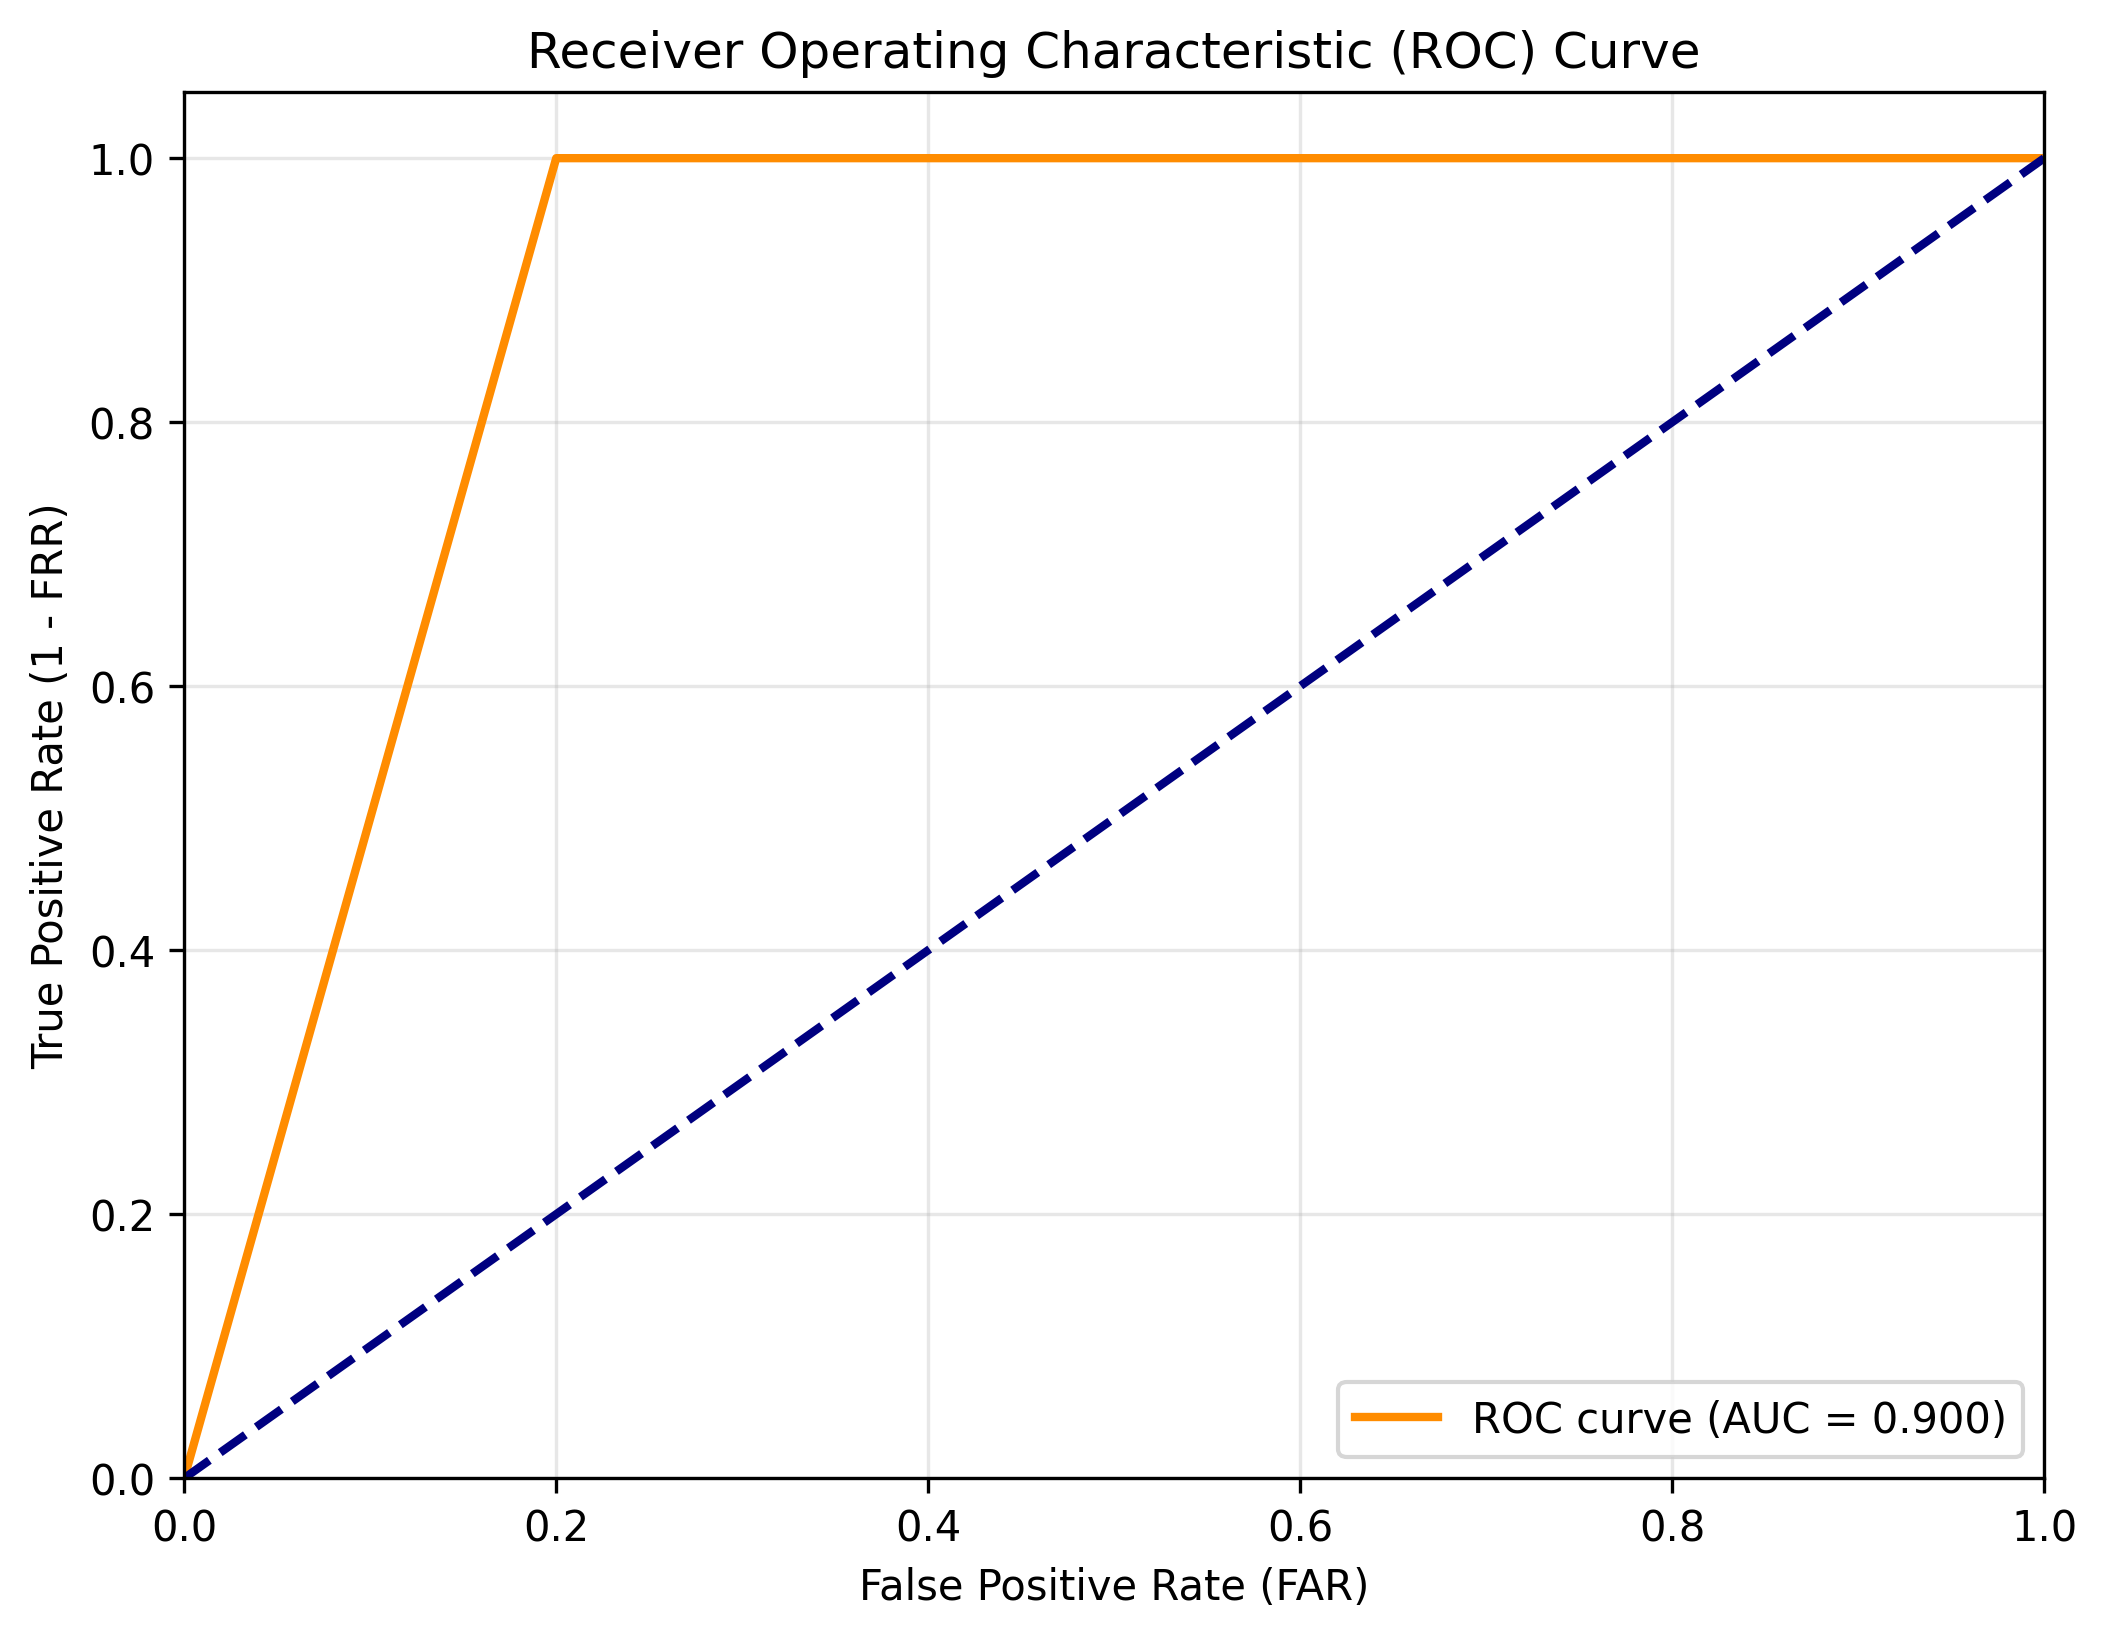
\includegraphics[width=0.72\linewidth]{../artifacts/capstone_eval/20260422T122948Z/roc_siamese.png}
\caption{ROC curve from the April 22, 2026 Siamese evaluation artifact}
\label{fig:roc}
\end{figure}

\begin{figure}[H]
\centering
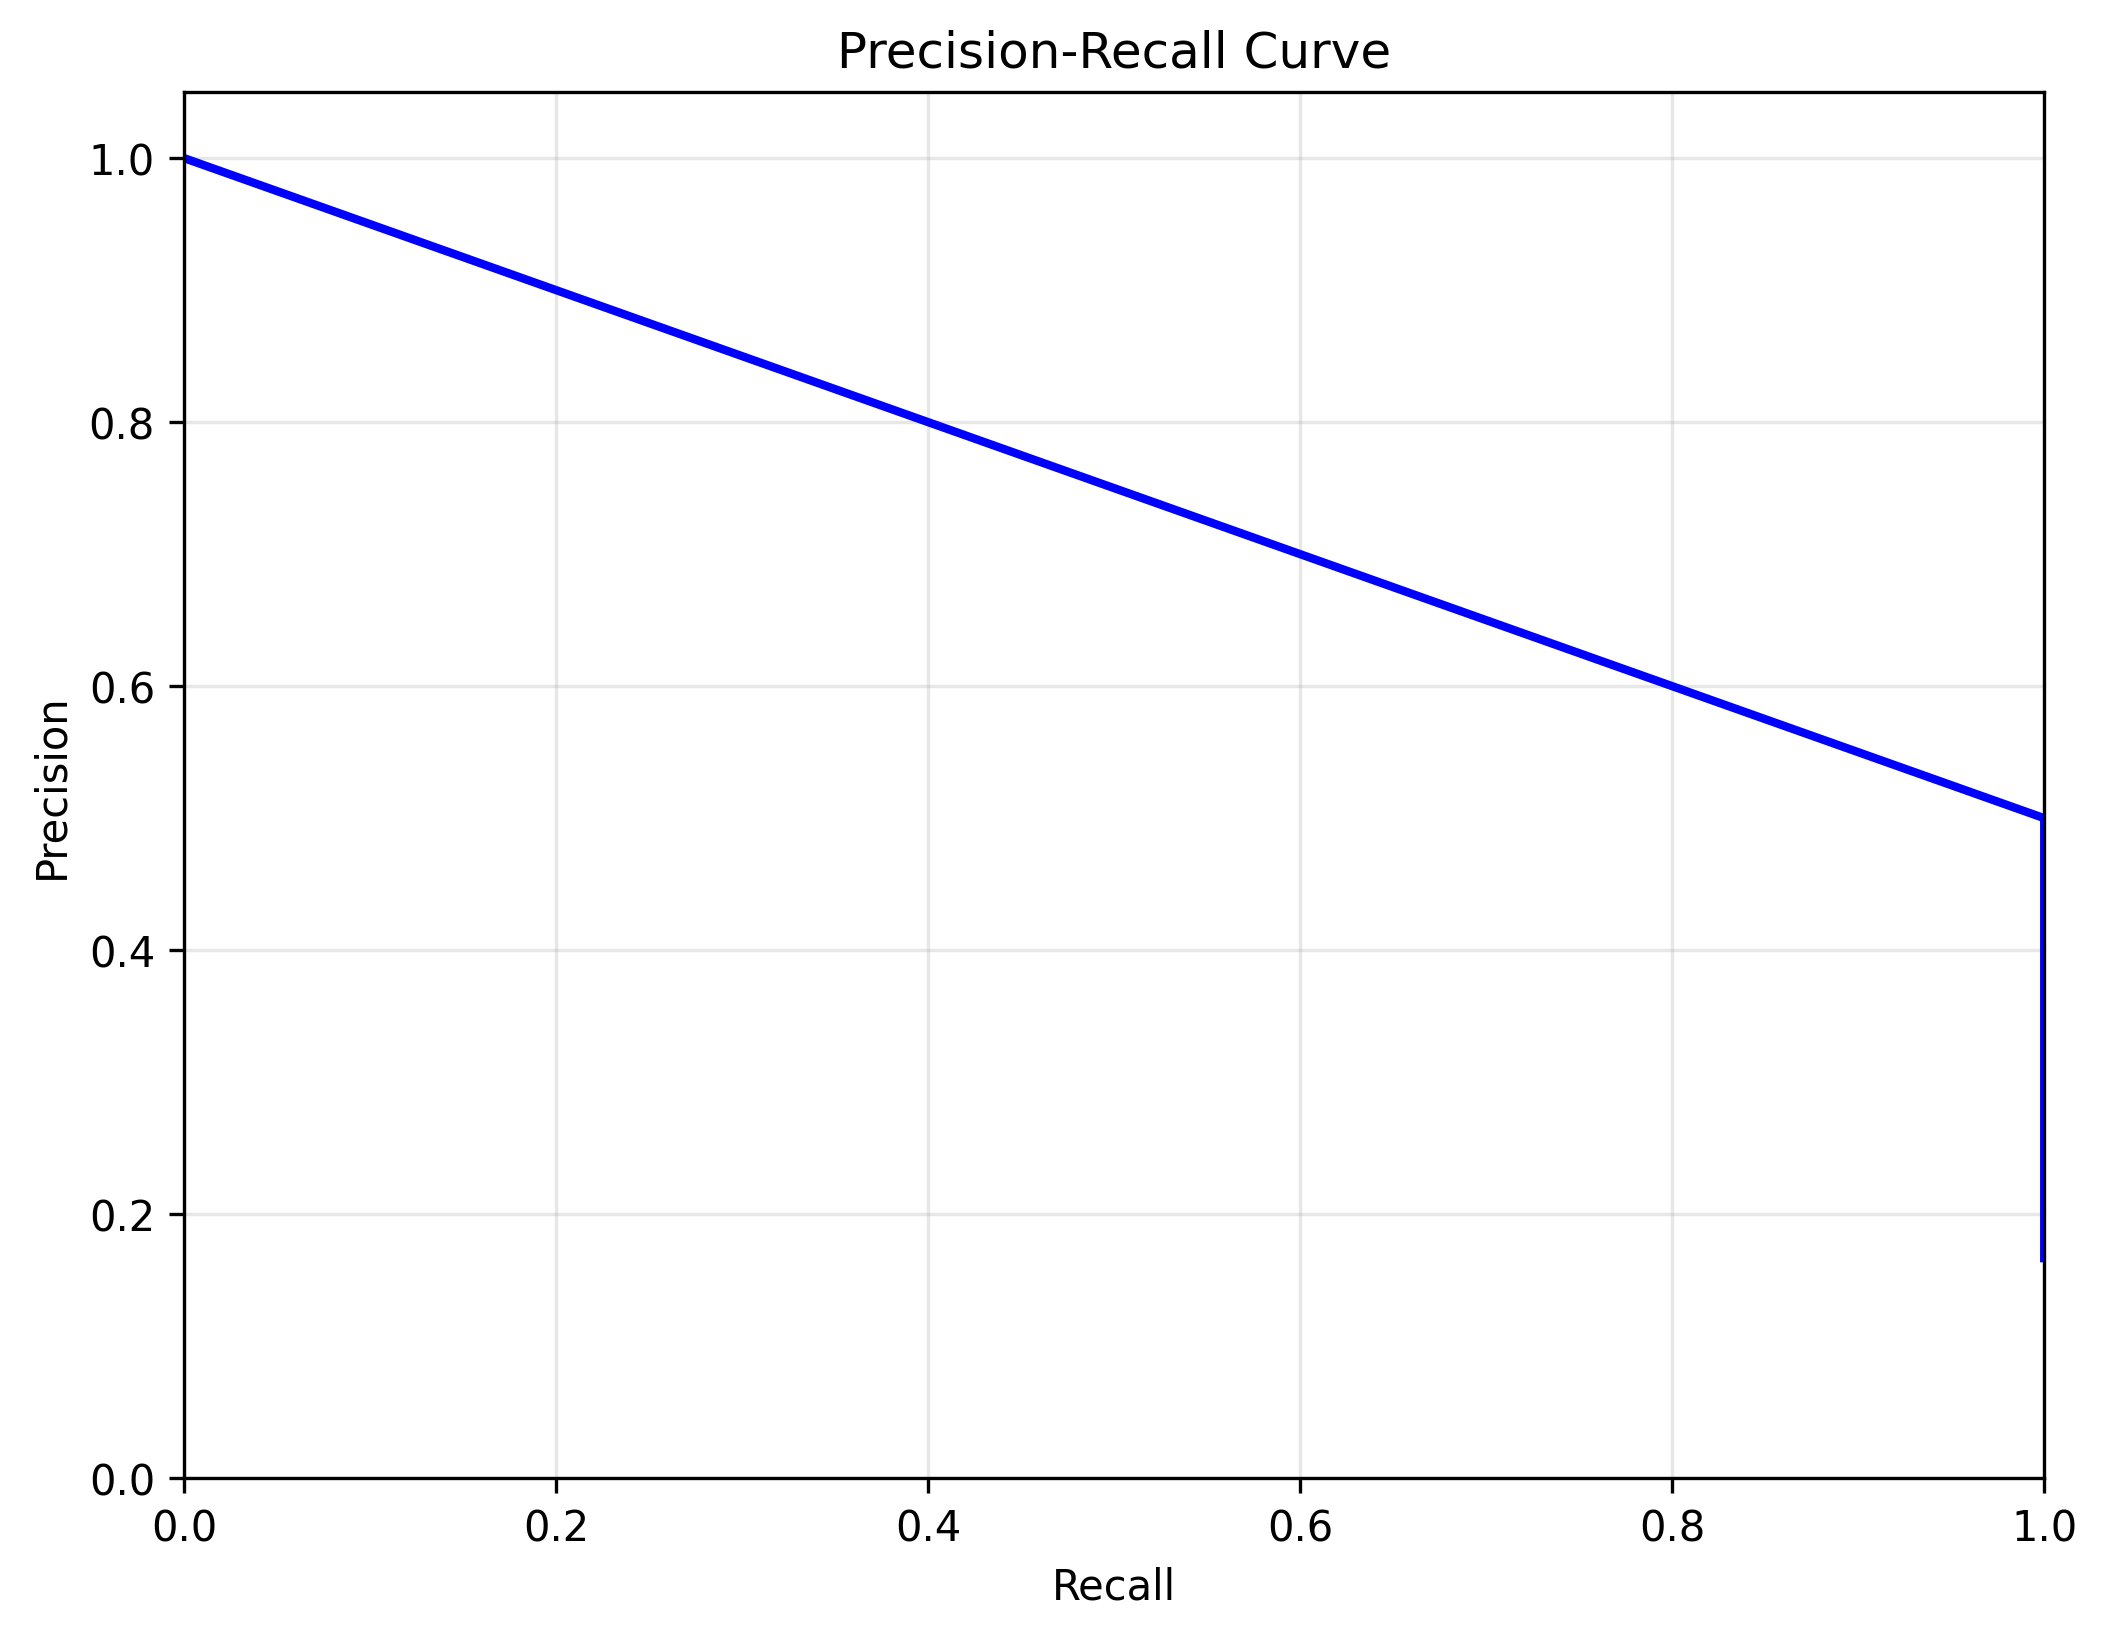
\includegraphics[width=0.72\linewidth]{../artifacts/capstone_eval/20260422T122948Z/pr_siamese.png}
\caption{Precision-recall curve from the April 22, 2026 Siamese evaluation artifact}
\label{fig:pr}
\end{figure}

\section{Discussion}
Three points emerge from the results.

First, the learned embedding approach is operationally meaningful. The existence of device-level evaluation artifacts, thresholds, score distributions, and ROC/PR plots demonstrates that the repository has moved beyond a raw proof-of-concept. The system is capable of producing structured verification scores that can be tuned and explained.

Second, thresholding alone is not enough. The runtime design correctly adds confidence bands, per-source checks, and nearest-impostor margins. This is especially important because some older metrics in the repository show much higher FAR values under broader or noisier settings. A single threshold would make the system look better on paper than it behaves in practice.

Third, the attack narrative is carefully bounded. The artifact reports zero mean attack success for replay, impersonation, and synthetic-statistics attacks under that evaluation configuration. This is encouraging, but it should be presented as evidence within that setup, not as proof of strong real-world adversarial robustness. The documentation already supports that conservative interpretation, and the thesis should preserve it.

\section{Limitations}
The main limitations are:
\begin{itemize}[leftmargin=1.2cm]
\item limited dataset scale relative to research-grade biometric evaluation;
\item potential environmental drift across sessions and recording conditions;
\item no claim of liveness detection or resistance to adaptive learned mimicry;
\item reliance on commodity hardware capture that may be unstable during demos;
\item mixed results across older metric files, indicating the need for stronger calibration and broader validation.
\end{itemize}

These limitations do not invalidate the project. They define the boundary within which the results should be interpreted.

\section{Reviewer-Safe Interpretation}
The repository's review notes recommend language such as ``prototype device-verification pipeline'' and ``measured under our dataset and split policy.'' That recommendation is correct. The best interpretation of the results is that QNA-Auth demonstrates a technically coherent prototype with promising behavior under documented conditions, while still requiring more data and stronger longitudinal validation before stronger claims are justified.

\chapter{Conclusion and Further Enhancements}
\section{Conclusion}
This thesis presented QNA-Auth, a noise-based device verification prototype that combines camera and microphone sensor fingerprints, engineered feature extraction, Siamese-style embeddings, and security-aware application logic. The project is noteworthy not because it proves perfect identity from noise, but because it builds a full verification system around realistic assumptions and careful claim boundaries.

The implemented pipeline performs multi-source enrollment, weighted similarity fusion, confidence-band classification, nearest-impostor margin checking, drift-aware template updates, and nonce-bound challenge verification. It also includes persistence, diagnostics, frontend support, evaluation artifacts, and reviewer-safe reporting. These features make the project suitable as a capstone thesis because they demonstrate not only modeling effort but also system design, operational thinking, and security awareness.

The current evidence suggests that sensor-noise-based verification can be a useful additional signal for high-confidence device matching under controlled conditions. The repository already contains one strong artifact slice and several supporting evaluation tools. At the same time, the system remains a prototype, and that limitation is central to an honest academic conclusion.

\section{Further Enhancements}
The most valuable next steps are:
\begin{itemize}[leftmargin=1.2cm]
\item build a larger multi-session dataset with stronger device diversity;
\item evaluate camera-only, microphone-only, and fused-source settings under identical split policies;
\item calibrate thresholds per environment or deployment profile instead of using one static global value;
\item introduce stronger anti-spoofing or liveness cues;
\item move challenge persistence and audit storage to a production-ready database configuration;
\item add secure client-assisted challenge computation if a stronger possession claim is needed;
\item quantify long-term drift using score distributions across days or weeks.
\end{itemize}

If these extensions are completed, the project could move from a capstone-grade prototype toward a more substantial research contribution in device verification.

\appendix

\chapter{Selected API Examples}
This appendix provides a compact reference for thesis readers and reviewers.

\begin{lstlisting}[language={},caption={Enrollment request example}]
{
  "device_name": "Lab Demo Laptop",
  "num_samples": 10,
  "sources": ["camera", "microphone"]
}
\end{lstlisting}

\begin{lstlisting}[language={},caption={Authentication response example with diagnostics}]
{
  "authenticated": true,
  "device_id": "abc123",
  "similarity": 0.982,
  "details": {
    "confidence_band": "strong_accept",
    "recommended_action": "accept",
    "observed_margin": 0.041,
    "margin_check_passed": true,
    "per_source_check_passed": true
  }
}
\end{lstlisting}

\chapter{Repository Mapping}
Table \ref{tab:repomap} maps the main thesis sections to repository locations.

\begin{longtable}{p{0.28\textwidth}p{0.62\textwidth}}
\caption{Repository locations relevant to the thesis}\label{tab:repomap}\\
\toprule
\textbf{Path} & \textbf{Role in the project} \\
\midrule
\endfirsthead
\toprule
\textbf{Path} & \textbf{Role in the project} \\
\midrule
\endhead
\texttt{server/app.py} & API startup, endpoints, runtime state, rate limiting, and orchestration \\
\texttt{auth/enrollment.py} & Enrollment logic, template creation, metadata, and drift updates \\
\texttt{auth/authentication.py} & Similarity scoring, source checks, confidence bands, margin guard \\
\texttt{auth/challenge\_response.py} & Nonce-bound challenge verification and HKDF hardening \\
\texttt{preprocessing/features.py} & Canonical feature pipeline shared by training and runtime \\
\texttt{model/siamese\_model.py} & Embedding network, losses, and similarity operations \\
\texttt{model/evaluate.py} & Threshold sweeps, EER, ROC, PR, and reporting \\
\texttt{db/models.py} & SQLAlchemy schemas for devices, challenges, and audit logs \\
\texttt{frontend/src/} & User interface pages and API client \\
\texttt{artifacts/capstone\_eval/20260422T122948Z} & Latest included evaluation artifact used in this report \\
\texttt{docs/DEMO\_RUNBOOK.md} & Review-day live demo and fallback flow \\
\texttt{docs/REVIEW\_SLIDE\_NOTES.md} & Reviewer-safe wording and presentation narrative \\
\bottomrule
\end{longtable}

\begin{thebibliography}{99}
\bibitem{bromley1993signature}
Jane Bromley, Isabelle Guyon, Yann LeCun, Eduard Sackinger, and Roopak Shah.
\newblock Signature verification using a ``Siamese'' time delay neural network.
\newblock In \emph{Advances in Neural Information Processing Systems}, 1993.

\bibitem{hadsell2006dimensionality}
Raia Hadsell, Sumit Chopra, and Yann LeCun.
\newblock Dimensionality reduction by learning an invariant mapping.
\newblock In \emph{Proceedings of the IEEE Conference on Computer Vision and Pattern Recognition}, 2006.

\bibitem{schroff2015facenet}
Florian Schroff, Dmitry Kalenichenko, and James Philbin.
\newblock FaceNet: A unified embedding for face recognition and clustering.
\newblock In \emph{Proceedings of the IEEE Conference on Computer Vision and Pattern Recognition}, 2015.

\bibitem{shannon1948mathematical}
Claude E. Shannon.
\newblock A mathematical theory of communication.
\newblock \emph{Bell System Technical Journal}, 27(3):379--423, 1948.

\bibitem{welch1967use}
Peter D. Welch.
\newblock The use of fast Fourier transform for the estimation of power spectra.
\newblock \emph{IEEE Transactions on Audio and Electroacoustics}, 15(2):70--73, 1967.

\bibitem{goodfellow2016deep}
Ian Goodfellow, Yoshua Bengio, and Aaron Courville.
\newblock \emph{Deep Learning}.
\newblock MIT Press, 2016.
\end{thebibliography}

\end{document}
